%------------------------------------------------
%	PACKAGES AND THEMES
%------------------------------------------------

% this is a 4:3 layout.
\documentclass{beamer}
% for 16:9 use this command:
% \documentclass[aspectratio=169]{beamer}

\mode<presentation> {
\usetheme{metropolis}
\setbeamertemplate{caption}[numbered]
\setbeamertemplate{navigation symbols}{} % hide navigation symbols
}

\usepackage{graphicx} % images
\usepackage{algorithm2e}
\usepackage{mathtools}
\DeclarePairedDelimiter{\ceil}{\lceil}{\rceil}
\usepackage{algpseudocode}
\usepackage{booktabs} % allows the use of \toprule, \midrule and \bottomrule in tables
\usepackage[ngerman]{babel}
\usepackage[utf8]{inputenc}
\usepackage[T1]{fontenc}
\usepackage{mathtools}
\usepackage{xcolor}
\usepackage{listings} % code
\usepackage{pgf,tikz} % drawing
\usepackage{pifont} % new symbols
\usepackage{hyperref} % pretty links
% \usepackage{algorithmicx}
% \usepackage{algpseudocode}
% \usepackage[linesnumbered,ruled]{algorithm2e}

\usepackage{lmodern}
\usepackage{subcaption}
\usepackage{textcomp}
% \usepackage{array}
% \usepackage{longtable}
% \usepackage{verbatim}
%\usepackage{tabularx}
\captionsetup[figure]{font=footnotesize}

\usepackage{amsmath}
\usepackage{amssymb}
\usepackage{amsthm}
% \usepackage{comment}
% \usepackage{enumitem}
% \usepackage[binary-units=true]{siunitx}
% \usepackage{thmtools}
\usepackage{csquotes}
\usepackage{tikz}
\usepackage{float}
\usetikzlibrary{automata,positioning}

% color settings for links
\hypersetup{
    colorlinks=true,
    urlcolor=blue,
    linkcolor=black,
    citecolor=green!50!black
}

\definecolor{mygreen}{RGB}{1,135,1}

\newcommand{\cmark}{\ding{51}}  % checkmark
\newcommand{\xmark}{\ding{55}}  % xmark
\newcommand\scalemath[2]{\scalebox{#1}{\mbox{\ensuremath{\displaystyle #2}}}}

\setbeamerfont{bibliography item}{size=\footnotesize}
\setbeamerfont{bibliography entry author}{size=\footnotesize}
\setbeamerfont{bibliography entry title}{size=\footnotesize}
\setbeamerfont{bibliography entry location}{size=\footnotesize}
\setbeamerfont{bibliography entry note}{size=\footnotesize}

% \useoutertheme{miniframes} % navigation design
\useinnertheme{circles} % use non shiny circles (itemize, etc.)

% Main slide colors
% dunkel, hell, mittel
% \definecolor{pale}{RGB}{232, 236, 237}
% \definecolor{prim}{RGB}{53, 109, 120}
% \definecolor{sec}{RGB}{104, 170, 183}
% \definecolor{tert}{RGB}{109, 155, 168}
% \definecolor{quat}{RGB}{9, 59, 68}

\definecolor{pale}{RGB}{255, 255, 255}
% \definecolor{prim}{RGB}{153, 194, 173}
% good: \definecolor{prim}{RGB}{27, 33, 42}
\definecolor{prim}{RGB}{32, 43, 50}
\definecolor{sec}{RGB}{217, 232, 224}
\definecolor{tert}{RGB}{0, 82, 41}
% save
\definecolor{quat}{RGB}{0, 82, 41}

\setbeamercolor{palette primary}{bg=prim,fg=pale}
\setbeamercolor{palette secondary}{bg=sec,fg=pale}
\setbeamercolor{palette tertiary}{bg=tert,fg=pale}
\setbeamercolor{palette quaternary}{bg=quat,fg=pale}
\setbeamercolor{structure}{fg=prim} % itemize, enumerate, etc
\setbeamercolor{section in toc}{fg=prim} % TOC sections

% Block colors
\definecolor{example_color}{RGB}{93, 137, 98}
\definecolor{alert_color}{RGB}{175, 79, 72}

\setbeamercolor{normal text}{fg=prim!20!black,bg=pale!25!white}
\setbeamercolor{alerted text}{fg=alert_color!25!black}
\setbeamercolor{example text}{fg=example_color!25!black}

\setbeamercolor{block title example}{fg=white,bg=example_color}
\setbeamercolor{block body example}{fg=black,bg=example_color!10!white}
\setbeamercolor{block title alerted}{fg=white,bg=alert_color}
\setbeamercolor{block body alerted}{fg=black,bg=alert_color!10!white}

% Override palette coloring
\setbeamercolor{subsection in head/foot}{bg=quat,fg=pale}

\setbeamertemplate{frametitle}{%
    \nointerlineskip%

    \begin{beamercolorbox}[wd=\paperwidth,ht=2.5ex,dp=1ex]{frametitle}
        \hspace*{1ex}\insertframetitle%
        \ifx\insertframesubtitle@empty\else%
        {~\tiny\textcolor{quat!35!black}{\insertframesubtitle}}%
        \fi%
    \end{beamercolorbox}%
}

% math-command for bigger norm
\newcommand\norm[1]{\left\lVert#1\right\rVert}

% use this to include other files
% in this case style definitions for code
% alternative: \include{dateiname}
\lstdefinestyle{latex}{
    language=[LaTeX]TeX,
    inputencoding=utf8,
    basicstyle=\ttfamily,
    keywordstyle=\color{blue!60!black}, % use 60 percent blue and 40 black
    commentstyle=\color{cyan!60!black},
    tabsize=2,
    emph={document,itemize,enumerate,center,tabular,table,
    figure,wrapfigure,minipage,columns,align,bmatrix,
    lstlisting,beamer,frame,tikzpicture},
    emphstyle=\color{magenta!60!black},
    morekeywords={lstset,includegraphics,theenumi,labelitemi,column,color,url,href}
}

\lstdefinestyle{inline_latex}{
    language=[LaTeX]TeX,
    inputencoding=utf8,
    basicstyle=\ttfamily,
    resetmargins= true,
    belowcaptionskip=0pt,
    aboveskip=0pt,
    belowskip=0pt,
    keywordstyle=\color{blue!60!black},
    commentstyle=\color{cyan!60!black},
    emph={document,itemize,enumerate,center,tabular,table,
    figure,wrapfigure,minipage,columns,align,bmatrix,
    lstlisting,beamer,frame,tikzpicture,Parameter},
    emphstyle=\color{magenta!60!black},
    morekeywords={lstset,includegraphics,theenumi,labelitemi,column,color,url,href,Befehlsname}
}

\lstdefinestyle{cpp}{
    language=C++,
    basicstyle=\ttfamily,
    keywordstyle=\color{blue!90!black},
    stringstyle=\color{magenta!60!black},
    commentstyle=\color{green!35!black},
    morecomment=[l][\color{gray!60!black}]{\#},
    tabsize=2
}

\lstdefinestyle{empty}{
    basicstyle=\rmfamily,
    keywordstyle=\bfseries,
    commentstyle=\color{black}\itshape
}

\lstset{style=latex}

%------------------------------------------------
%	TITLE PAGE
%------------------------------------------------

\selectlanguage{ngerman}
\title[]{Robustness \& Graph (Convolutional) Neural Networks}

\author{Tim Bohne}
\institute[]
{
\textit{Machine Learning Seminar 20/21}
\medskip
}
\date{\today}

% make slide at the beginnig of each section
\AtBeginSection[]{
{\setbeamercolor{background canvas}{bg=white}}}

% where images are locatied
\graphicspath{{./images/}}

\begin{document}

\begin{frame}[plain] % plain slides dont have navigation bars etc.
\titlepage % Print the title page as the first slide
\end{frame}

\begin{frame}
\frametitle{Übersicht} % table of contents slide
\tableofcontents
\end{frame}

%------------------------------------------------
\section{Motivation}
%------------------------------------------------

\begin{frame}
  \frametitle{Motivation}
  \textbf{Motivationen für Graph Neural Networks:}
  \begin{enumerate}
    \item Convolutional Neural Networks (CNNs)
    \item Graph Embedding
  \end{enumerate}
\end{frame}

\begin{frame}
  \frametitle{Convolutional Neural Networks (CNNs)}
  \begin{figure}
    \centering
    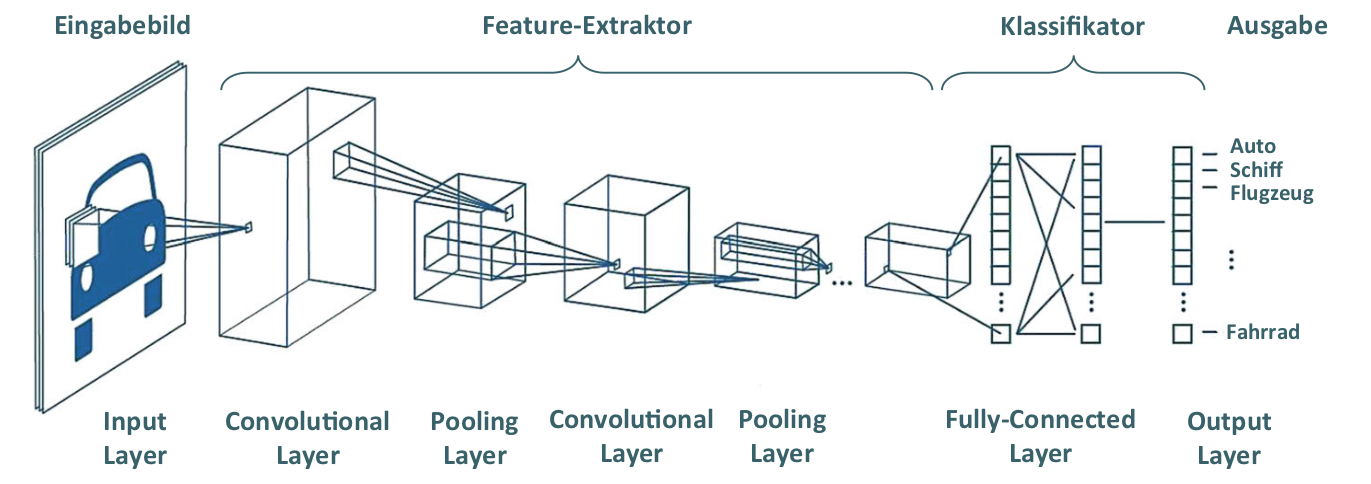
\includegraphics[width=\textwidth]{img/CNN.png}
    \caption*{Convolutional Neural Network \cite{Zschech2020}}
  \end{figure}
  \begin{itemize}
    \item \textbf{Feature-Learning}\newline Sequenz aus Convolutional- und Pooling-Layern
    \item \textbf{Classification}
  \end{itemize}
\end{frame}

\begin{frame}
  \frametitle{Convolutional Neural Networks (CNNs)}
  \begin{figure}
    \centering
    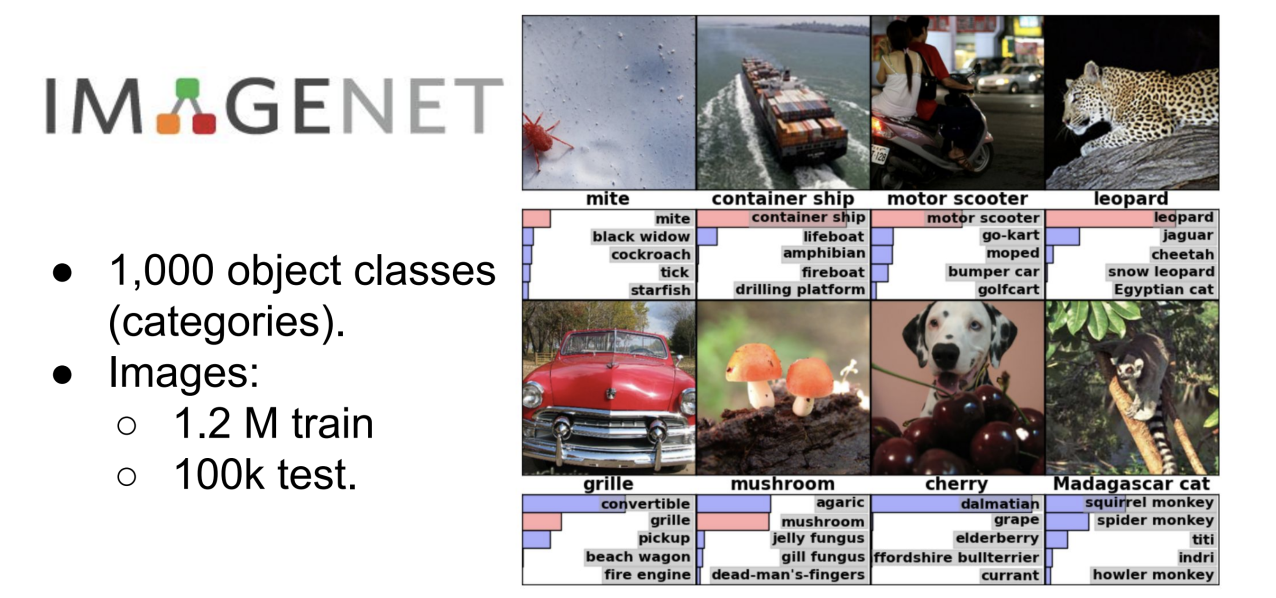
\includegraphics[width=\textwidth]{img/imagenet.png}
    \caption*{ImageNet Challenge \cite{Giro-o-Nieto}}
  \end{figure}
  Hier sind CNNs sehr erfolgreich!
\end{frame}

\begin{frame}
  \frametitle{Convolutional Neural Networks (CNNs)}
  \textbf{Problem}: CNNs funktionieren lediglich mit Euklidischen Datenstrukturen (Bilder, Text), nicht mit Graphen!
  
    \begin{figure}[H]
      \centering
      \begin{subfigure}[b]{0.49\textwidth}
        \centering
        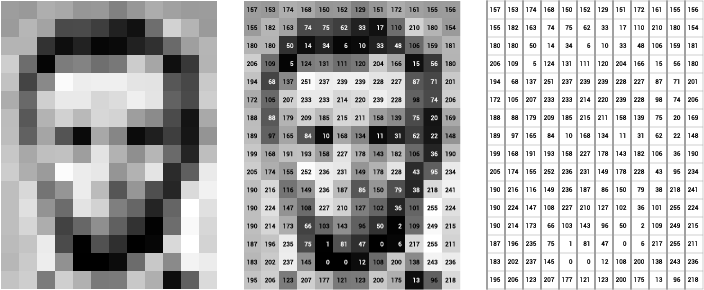
\includegraphics[width=\textwidth]{img/pixelmatrix.png}
        \caption*{Pixelmatrix \cite{PixelMatrix}}
      \end{subfigure}
      \begin{subfigure}[b]{0.49\textwidth}
        \centering
        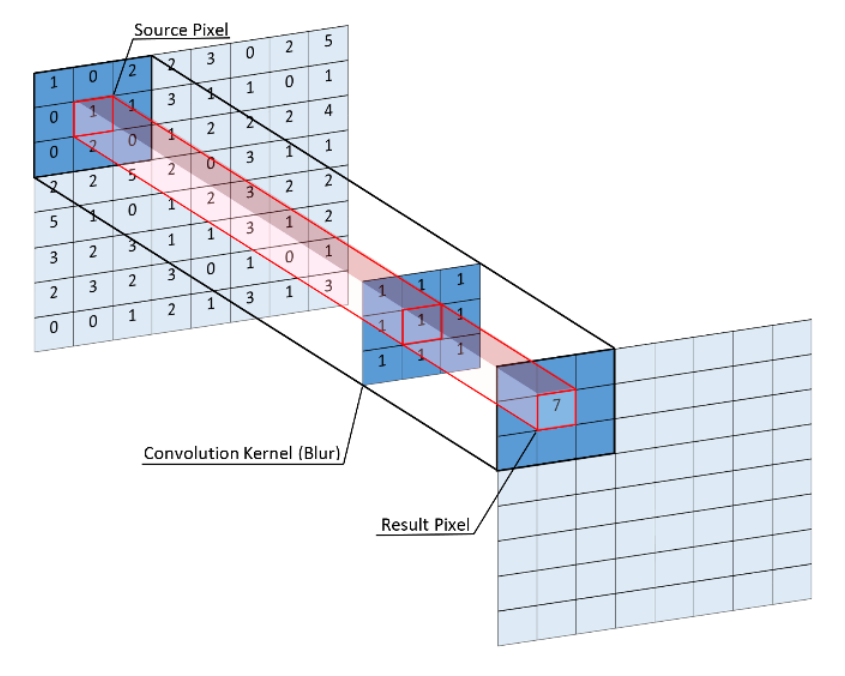
\includegraphics[width=\textwidth]{img/convolution.png}
        \caption*{Convolution-Operation \cite{Convolution}}
      \end{subfigure}
    \end{figure}
\end{frame}

\begin{frame}
  \frametitle{Graph Embedding}
  \textbf{Übersetze Graph-Struktur in niedrigdimensionalen Vektor}
  \begin{figure}
    \centering
    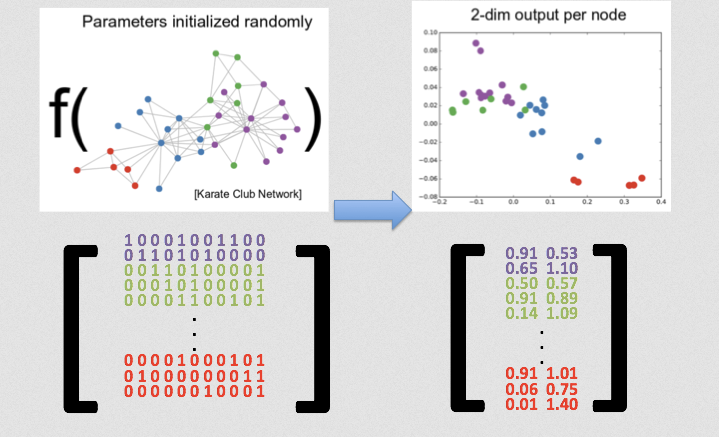
\includegraphics[width=\textwidth]{img/graph_embedding.png}
    \caption*{2-dim. Output für jeden Knoten \cite{Perozzi_2014}}
  \end{figure}
\end{frame}

%------------------------------------------------
\section{Graph Neural Networks (GNNs)}
%------------------------------------------------

\begin{frame}
  \frametitle{Graph Neural Networks (GNNs)}
  \textbf{Ermöglichen Machine Learning auf Graphen, z.B.:}
  \begin{itemize}
    \item Modellierung physikalischer Systeme
    \item Lernen molekularer Fingerabdrücke
    \item Analyse sozialer Netzwerke (Vorhersagen / Empfehlungen)
    \item Empfehlungssysteme
  \end{itemize}
  \begin{figure}
    \centering
    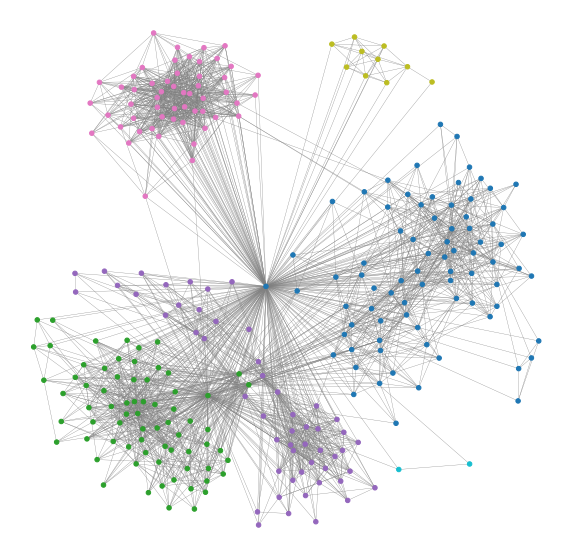
\includegraphics[width=0.4\textwidth]{img/social_graph.png}
    \caption*{Freunde-Netzwerk einer Person \cite{Facebook}}
  \end{figure}
\end{frame}

\begin{frame}
  \frametitle{Graph Neural Networks (GNNs)}
  \textbf{Typische Aufgaben für GNNs:}
  \begin{itemize}
    \item Semi-Supervised Node Classification
    \item Graph Classification
    \item Link Prediction
    \item Clustering
  \end{itemize}
\end{frame}

\begin{frame}
  \frametitle{Graph Neural Networks (GNNs)}
  Graph $\boldsymbol{G = (X, A)}$\newline
  $\boldsymbol{X}:$ Knoten - Personen in sozialem Netzwerk\newline
  $\boldsymbol{A}:$ Kanten - Beziehungen zwischen Personen
  \begin{figure}
    \centering
    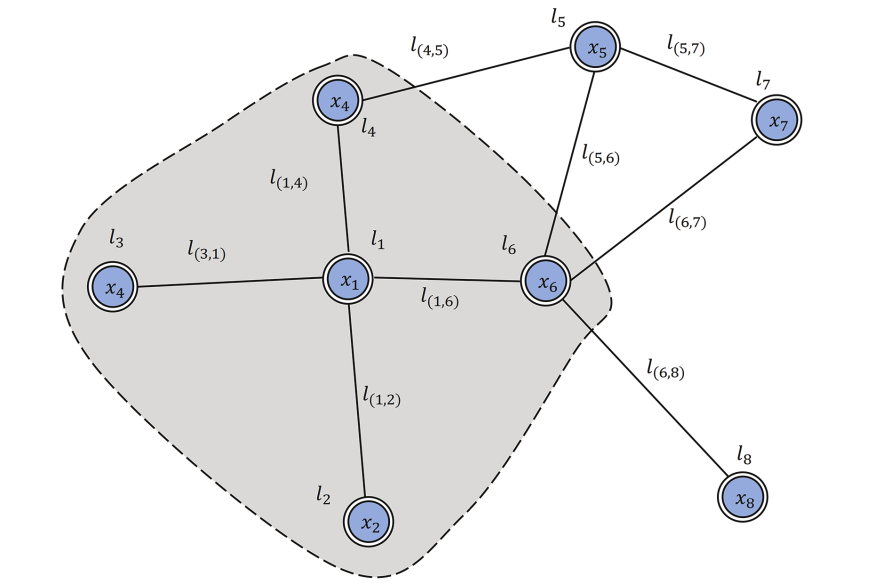
\includegraphics[width=0.575\textwidth]{img/graph.png}
    \caption*{Graph basierend auf Scarselli et al. \cite{Liu_2020}}
  \end{figure}
  \textbf{Ziel}: Lerne Node Embedding $\boldsymbol{h_v}$ für jeden Knoten $\boldsymbol{v} \in \boldsymbol{X}$ um 
  einen Output $\boldsymbol{o_v}$ zu generieren, z.B. das vorhergesagte Label
\end{frame}

\begin{frame}
  \frametitle{Graph Neural Networks (GNNs)}

  $2$ wichtige Funktionen ($x$: Input Feature, $h$: Hidden State):
  \begin{enumerate}
    \item \textbf{Node Embedding:} $\quad\quad h_v = f(x_v, x_{co[v]}, h_{ne[v]}, x_{ne[v]})$
    \item \textbf{Output Embedding:} $\quad\thinspace o_v = g(h_v, x_v)$
  \end{enumerate}

  \underline{Lerne Parameter von $f$ und $g$:}

  \textbf{Loss Term:} $\sum_{i=1}^p (t_i - o_i)$

  \textbf{Lernmethode}: Gradient Descent
  \begin{itemize}
    \item Iteratives State-Update: $H^{t+1} = F(H^t, X)$
    \item Gradient der Gewichte $W$ wird basierend auf Loss berechnet
    \item Gewichte $W$ werden basierend auf dem Gradienten adaptiert
  \end{itemize}
\end{frame}

\begin{frame}
  \frametitle{Graph Convolutional Networks (GCNs)}

  \textbf{Input:} Features $X$, Adjazenzmatrix $A$\newline
  \textbf{Output:} Feature-Vektor für jeden Knoten
  \begin{figure}
    \centering
    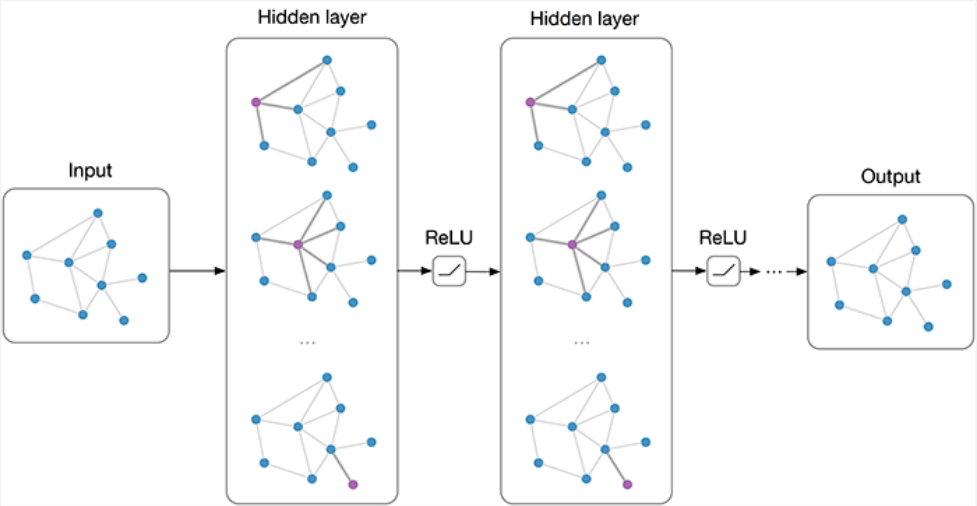
\includegraphics[width=0.75\textwidth]{img/GCN.png}
    \caption*{Multi-Layer GCN \cite{Kipf_2016}}
  \end{figure}
  \textbf{Anschließend Node Classification basierend auf den Output-Features}
\end{frame}

\begin{frame}
  \frametitle{Graph Convolutional Networks (GCNs)}

  Standard Convolution kann nicht für Graphen definiert werden!\newline
  \textbf{Lösung}: Embeddings (spectral / spatial)\newline

  \textbf{Approximierte \textquote{Graph-Convolution}} (Kipf et al. \cite{Kipf_2016}):\newline
  $\boldsymbol{H^{(l+1)} = \sigma [\hat{D}^{- \frac{1}{2}} \hat{A} \hat{D}^{- \frac{1}{2}} H^{(l)} W^{(l)}]}$\newline

  Sehr erfolgreich in praktischen Anwendungen eingesetzt!
\end{frame}

%------------------------------------------------
\section{Robustheit}
%------------------------------------------------

\begin{frame}
  \frametitle{Robustheit von Machine Learning Modellen}

  \textbf{Machine Learning Modelle sind i.A. anfällig für \textquote{Adversarial Attacks}}

  \begin{figure}
    \centering
    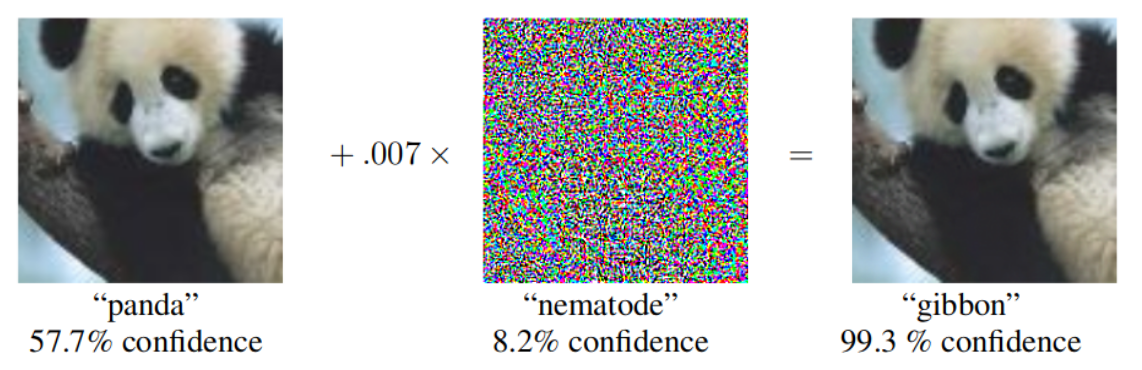
\includegraphics[width=\textwidth]{img/adversarial.png}
    \caption*{Adaptiert aus Goodfellow et al. \cite{Goodfellow_2015}}
  \end{figure}
\end{frame}

\begin{frame}
  \frametitle{Robustheit von GNNs}
  Dies gilt auch für GNNs, wobei sich zwei Arten von Angriffen unterscheiden lassen:
  \begin{itemize}
    \item \textbf{Manipulation der Knoten-Attribute}
    \item \textbf{Manipulation der Graph-Struktur}
  \end{itemize}
  \begin{figure}
    \centering
    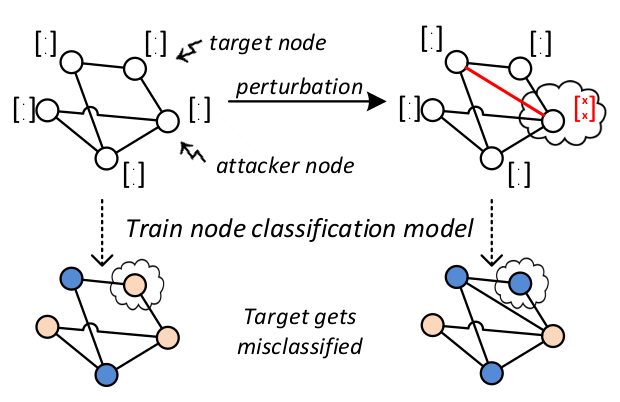
\includegraphics[width=0.7\textwidth]{img/adversarial_GNN.png}
    \caption*{Zügner et al. \cite{Zuegner_2018}}
  \end{figure}
\end{frame}

\begin{frame}
  \frametitle{Robustheit von GNNs}
  \textbf{3 Phasen in der Literatur:}
  \begin{enumerate}
    \item GNNs anfällig für \textquote{Adversarial Attacks}
    \item Verteidigungsmechanismen für konkrete Szenarien
    \item Beweisbare Garantien für die Robustheit bestimmter Modelle
  \end{enumerate}
\end{frame}

\begin{frame}
  \frametitle{Semi-Supervised Node Classification}

  Graph $\boldsymbol{G} = (\boldsymbol{A}, \boldsymbol{X})$ $\quad$ Zielknoten $\boldsymbol{t}$ $\quad$ Trainierbare Parameter $\boldsymbol{\theta}$\newline
  $\boldsymbol{A}$: Adjazenzmatrix, $\boldsymbol{X}$: Knoten-Features\newline

  $\boldsymbol{V}$: Knotenmenge\newline
  $\boldsymbol{V_L} \subseteq \boldsymbol{V}$: Teilmenge der gelabelten Knoten\newline

  $\boldsymbol{\mathcal{T}(A)}$: \textquote{Message-Passing-Matrix} - wie Aktivierungen durch das GNN propagiert werden
  $\rightarrow$ Transformation der Adjazenzmatrix\newline

  \textbf{Cross-Entropy-Loss Minimierung}:\newline
  Lerne $\boldsymbol{\theta}$ unter Verwendung der $\boldsymbol{V_L}$\newline

  \textbf{Ziel}: Label der verbleibenden Knoten ohne Label vorhersagen

\end{frame}

%------------------------------------------------
\subsection{GNNs: Manipulation der Knoten-Attribute}
%------------------------------------------------

\begin{frame}
  \frametitle{Robustheit von GNNs}
  \textbf{Zertifizierte Robustheit gegenüber Manipulationen der Knoten-Attribute} - Zügner et al. \cite{Zuegner_2019}\newline

  Wie lässt sich sicherstellen, dass kleine Änderungen an den Attributen keine dramatischen Auswirkungen auf den Output haben?
\end{frame}

\begin{frame}
  \frametitle{Zertifizierung der Robustheit bereits trainierter GNNs}

  \textbf{Ziel}: Zertifikat für Knoten $\boldsymbol{t}$ bedeutet, dass die Vorhersage für $\boldsymbol{t}$ sich nach zulässigen Manipulationen nicht ändert\newline
  $\rightarrow$ Definiertes Angriffsmodell\newline

  \textbf{Idee:}
  \textquote{\textbf{Worst-Case-Margin}} $\boldsymbol{m^t}$ für Knoten $\boldsymbol{t}$ zwischen den Klassen $\boldsymbol{y}$ und $\boldsymbol{y^{\ast}}$ 
  bzgl. zulässiger Manipulationen:
  \begin{gather} 
        \boldsymbol{m^t (y^*, y) := \min_{\tilde{X}} f_{\theta}^t(\tilde{X}, A)_{y^*} - f_{\theta}^t(\tilde{X}, A)_y} \nonumber \\
        \boldsymbol{s.t. \quad \tilde{X} \in zul. Manipulationen} \nonumber
  \end{gather}

  $\boldsymbol{m^t > 0 \thinspace \forall \thinspace y \neq y^{\ast}} \rightarrow $ Modell robust bzgl. Knoten $\boldsymbol{t}$

\end{frame}

\begin{frame}
  \frametitle{High-Level Idee}
  \begin{figure}[H]
    \centering
    \begin{subfigure}[b]{1\textwidth}
      \centering
      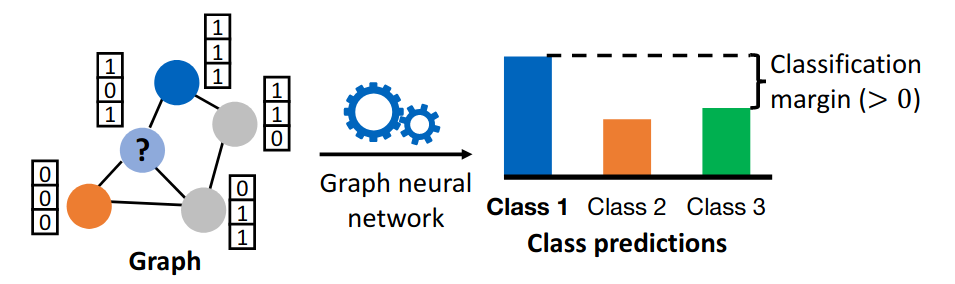
\includegraphics[width=0.75\textwidth]{img/before_pert.png}
      \caption*{Vor der Manipulation \cite{Zuegner_2019}}
    \end{subfigure}
    \par\bigskip
    \begin{subfigure}[b]{1\textwidth}
      \centering
      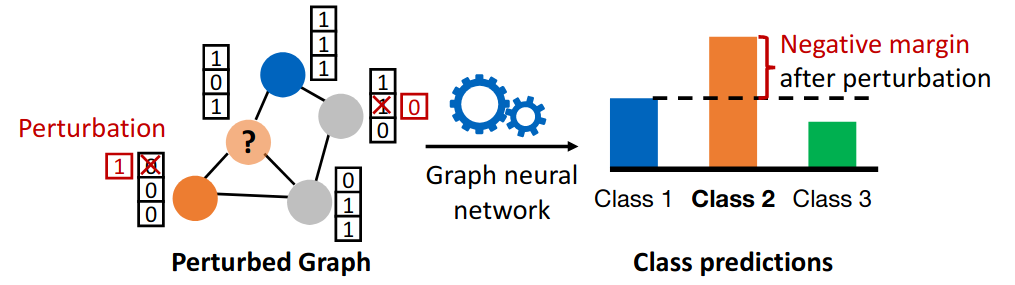
\includegraphics[width=0.75\textwidth]{img/after_pert.png}
      \caption*{Nach der Manipulation \cite{Zuegner_2019}}
    \end{subfigure}
  \end{figure}
\end{frame}

\begin{frame}
  \frametitle{Lösung des Optimierungsproblems}
  \textbf{Optimierungsproblem nicht effizient lösbar}:\newline 
  Diskrete Daten + nicht-konvexe Aktivierungsfunktion\newline

  \textbf{Lösung}:
  \begin{itemize}
    \item Konvexe ReLU Relaxation: Transformiert das GNN in ein effizient lösbares LP
    \item Kontinuierliche Relaxation der ganzzahligen Knotenattribute
  \end{itemize}

  $\rightarrow$ Effizient berechenbare Schranken für den Worst-Case-Margin\newline
  $\rightarrow$ Ggf. \textquote{false negatives}, jedoch keine \textquote{false positives}
\end{frame}

\begin{frame}
  \frametitle{Training mit dem Ziel der Robustheit}

  \textbf{Ziel}: Erreiche beweisbare Robustheit durch Training\newline
  $\rightarrow$ Optimiere bezüglich Robustheit

  \textbf{Robust Hinge Loss}
  \[
  \min_{\theta} \sum_{v \in V_L} \mathcal{L}(p_v, y_v) + \sum_{v \in V_L} \mathcal{\hat{L}}_{M_L} (-m^{\ast}_v, y_v)
  + \sum_{v \in V \backslash V_L} \mathcal{\hat{L}}_{M_U} (-m^{\ast}_v, \hat{y}_v)
  \]

  \begin{itemize}
    \item Relaxierte Version um Robustheit sicherzustellen
    \item Exakte Version für die Klassifizierung
  \end{itemize}  

  $\rightarrow$ \textbf{Mit Standardsoftware robuste GNNs trainieren}\newline
  $\rightarrow$ \textbf{Qualität der \textquote{Classification}-Ergebnisse nicht schlechter}
\end{frame}

\begin{frame}
  \frametitle{Training mit dem Ziel der Robustheit}
  \begin{figure}
    \centering
    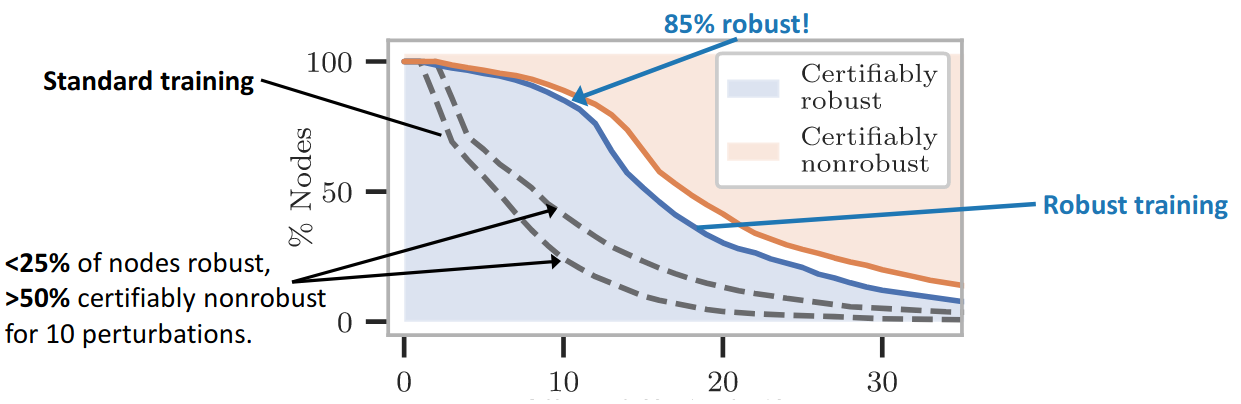
\includegraphics[width=\textwidth]{img/robust_training.png}
    \caption*{\textquote{Robustheits-Training} vs. Standard-Training \cite{Zuegner_2019}}
  \end{figure}
  \begin{itemize}
    \item Nur wenige Knoten nicht zertifizierbar
    \item Standard-Training führt zu GNNs, die nur robust bzgl. sehr weniger Manipulationen sind
  \end{itemize}
\end{frame}

%------------------------------------------------
\subsection{GNNs: Manipulation der Graph-Struktur}
%------------------------------------------------

\begin{frame}
  \frametitle{Robustheit von GNNs}
  \textbf{Zertifizierte Robustheit gegenüber Manipulationen der Graph-Struktur} - Zügner et al. \cite{10.1145/3394486.3403217}\newline

  Angreifer können neue Kanten in den Graphen einfügen, z.B. Likes in Social Media:
  \begin{figure}
    \centering
    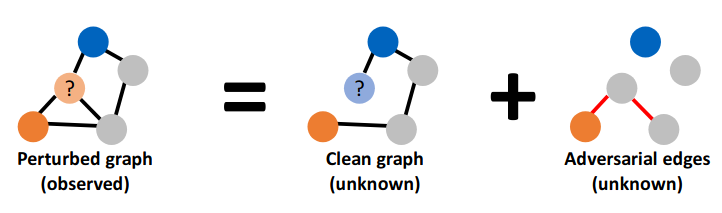
\includegraphics[width=\textwidth]{img/high_level_graph_pert.png}
    \caption*{High-Level Idee \cite{10.1145/3394486.3403217}}
  \end{figure}
\end{frame}

\begin{frame}
  \frametitle{Robustheit von GNNs}

  \textbf{Einfügen neuer Kanten kann die Vorhersagen des Modells ändern!}

  \textbf{Ziel:} Ein Zertifikat bedeutet, dass sich die Vorhersage für einen Knoten
  nicht ändert, wenn ein Angreifer Kanten hinzufügt.

  \textbf{Idee:} Prüfe, ob es einen Graphen gibt, der durch Entfernen von Kanten erreichbar ist und die Vorhersage ändert.

  \textbf{Angriffsmodell:} Praktisch unmöglich, alle Graphen zu enumerieren $\rightarrow$ Limitiere Anzahl an \textquote{Adversarial Edges}  
\end{frame}

\begin{frame}
  \frametitle{Optimierungsproblem}
  \begin{itemize}
    \item Bereits trainiertes GNN mit Parametern $\boldsymbol{\theta}$
    \item Input-Graph repräsentiert durch Matrix $\boldsymbol{A}$ möglicherweise manipuliert
    \item $\boldsymbol{A}$ ist von der \textquote{sauberen} Variante $\boldsymbol{A^{\ast}}$ durch eine Menge zulässiger Manipulationen der Graph-Struktur erreichbar
  \end{itemize}
  \textbf{Worst-Case-Margin:}
  \begin{gather}
    \boldsymbol{m^t (y^*, y) := \min_{\tilde{A}} f_{\theta}^t(X, \tilde{A})_{y^*} - f_{\theta}^t(X, \tilde{A})_y} \nonumber \\
    \boldsymbol{s.t. \quad \tilde{A} \in zul. Manipulationen} \nonumber
\end{gather}
  $\boldsymbol{m^t > 0 \thinspace \forall \thinspace y \neq y^{\ast}} \rightarrow $ Modell robust bzgl. Knoten $\boldsymbol{t}$
\end{frame}

\begin{frame}
  \frametitle{Optimierungsproblem}
  \textbf{Erneut nicht effizient lösbar!}\newline
  $\rightarrow$ Berechne LBs statt optimaler Zielfunktionswerte\newline

  \textbf{$3$ Schritte:}
  \begin{enumerate}
    \item Ersetzen der binären Adjazenzmatrix durch kontinuierliche Message-Passing-Matrix
    \item Relaxation der Aktivierungsfuntion des GNN
    \item Formulierung als \textquote{Jointly Constrained Bilinear Program} und Lösung durch Branch-and-Bound
    \begin{itemize}
      \item $LB > 0 \rightarrow$ robust
      \item $UB < 0 \rightarrow$ nicht entscheidbar
    \end{itemize}
  \end{enumerate}
\end{frame}

\begin{frame}
  \frametitle{Ergebnis}
  \begin{itemize}
    \item Effiziente Zertifizierung der Robustheit gegenüber Manipulationen der Graph-Struktur
    \item Bereits wenige Manipulationen führen zu einem Label-Wechsel eines beträchtlichen Anteils der Knoten
  \end{itemize}
  \begin{figure}
    \centering
    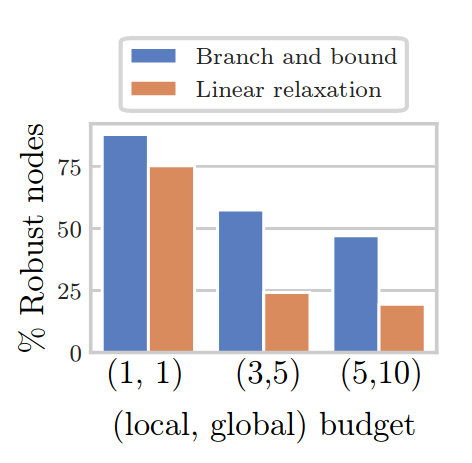
\includegraphics[width=0.5\textwidth]{img/graph_struct_pert_res.png}
    \caption*{B\&B vs. Lineare Relaxation \cite{10.1145/3394486.3403217}}
  \end{figure}
\end{frame}

%------------------------------------------------
\section{Fazit / Ausblick}
%------------------------------------------------

\begin{frame}
  \frametitle{Fazit}

  \begin{itemize}
    \item GNNs sind sehr \textbf{erfolgreich} in einer Vielzahl von praktischen Anwendungen einsetzbar
    \item GNNs sind \textbf{nicht robust} - anfällig für Manipulationen
    \begin{itemize}
      \item der Knoten-Attribute
      \item der Graph-Struktur
    \end{itemize}
    \item Um GNNs in (sicherheitskritischen) praktischen Anwendungen nutzen zu können, ist ein bestimmtes Maß an \textbf{Robustheit nötig}
    \item \textbf{Beweisbare Garantien} für die (Nicht-)Robustheit von GNNs sind möglich und nötig - erste Ansätze gesehen
  \end{itemize}
\end{frame}

\begin{frame}
  \frametitle{Ausblick}

  \begin{itemize}
    \item Spielraum für \textbf{Generalisierungen} (z.B. Angriffsmodelle)
    \item Trainingsmethoden, die \textbf{Robustheit explizit als Optimierungsziel} enthalten
    \item \textbf{Robustheitsgarantien} für Attribut- \underline{und} Struktur-Manipulationen
    \item \textbf{Grundsätzliches Verständnis} - was macht Manipulationen schädlich?
  \end{itemize}
\end{frame}

\begin{frame}
  \frametitle{Was macht Manipulationen schädlich?}

  \textbf{Ideen / Ansätze}
  \begin{itemize}
    \item Graphen, die reale Probleme repräsentieren besitzen bestimmte strukturelle Gemeinsamkeiten, die manipulierte Graphen verletzen
    \item Statistisch signifikante strukturelle Attribute in Manipulationen entdecken
    \item Wahrscheinlichkeit dafür, dass bestimmte gegebene Manipulationen schädlich sind
  \end{itemize}

  $\rightarrow$ \textbf{Allgemeinere Angriffsmodelle}\newline
  $\rightarrow$ \textbf{Manipulationen erkennen + verhindern}\newline
  $\rightarrow$ \textbf{Robustheit}\newline

\end{frame}

\begin{frame}[allowframebreaks]
  \bibliographystyle{plain}
  \bibliography{sources.bib}
\end{frame}

\end{document}
